\subsubsection{Information}
\begin{itemize}
	\item \textbf{Course Name:} \href{https://www.coursera.org/learn/foundations-user-experience-design}{Foundations of User Experience (UX) Design}
	\item \textbf{Instructor:} \href{https://www.coursera.org/instructor/google-career-certificates}{Google Career Certificates}
	\item \textbf{Level:} Beginner
	\item \textbf{Enrolled on:} March 14, 2024
	\item \textbf{Finished on:} April 4, 2024
	\item \textbf{Grade Achieved:} 95.56\%
\end{itemize}

\subsubsection{Certificate}
\begin{flushleft}
	\begin{figure}[!ht]
		\centering
		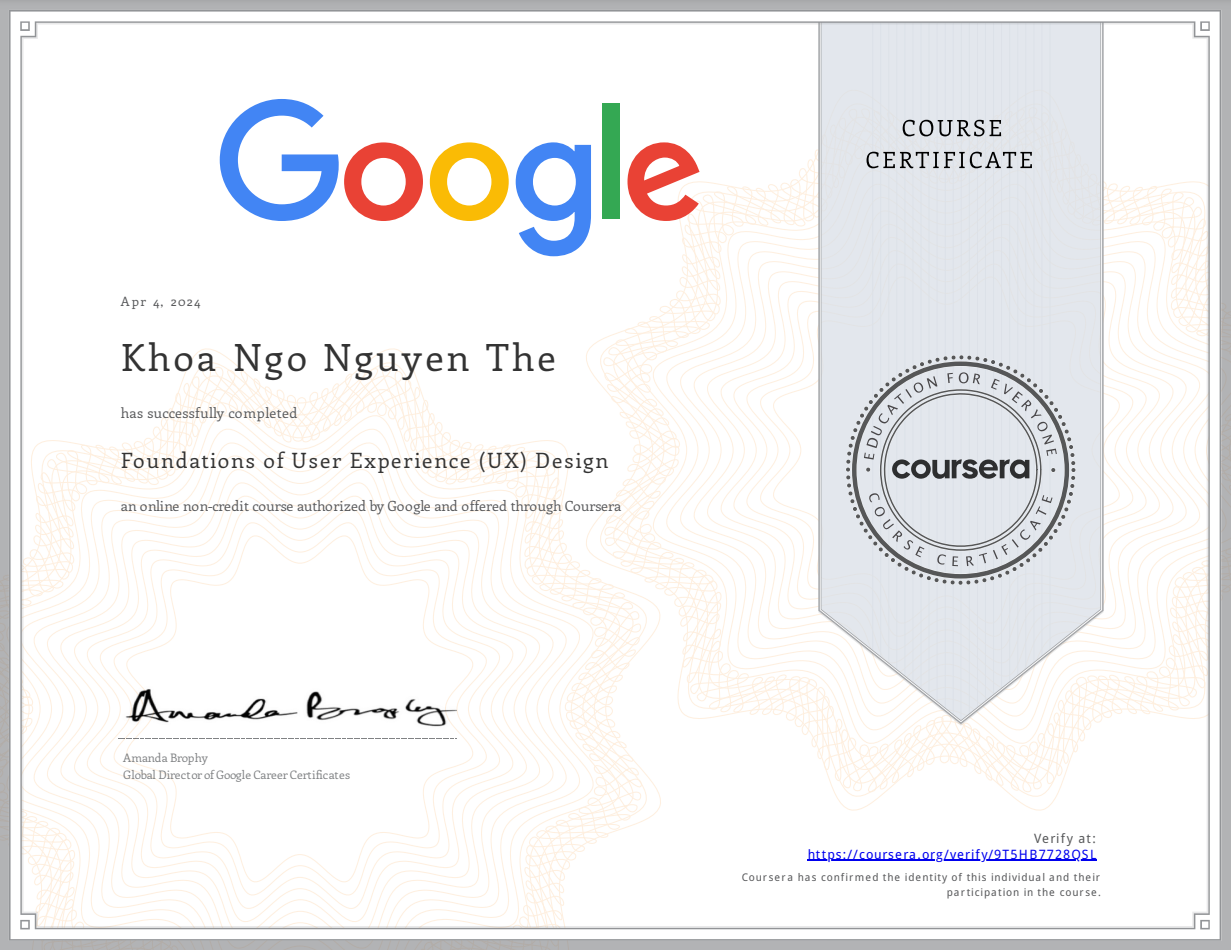
\includegraphics[width=0.85\textwidth]{imgs/Course1.png}
		\caption{Course 1 Certificate}
	\end{figure}

	Visit the online certificate for more info \href{https://www.coursera.org/account/accomplishments/verify/9T5HB7728QSL}{here}
\end{flushleft}

\subsubsection{Summary}
\begin{flushleft}
	What I have learned after completing this course:
	\begin{itemize}
		\item Identify common job responsibilities of entry-level UX designers and other teams I might work with.
		\item Understand foundational concepts in UX design, such as user-centered design, the design process, accessibility, and equity-focused design.
		\item Explain why design sprints are an important and useful part of a UX designer's work.
	\end{itemize}
\end{flushleft}

\subsubsection{Details}
\begin{flushleft}
	\begin{description}
		\item[Module 1:] Introducing User Experience Design
		      \begin{itemize}
			      \item I have been introduced to the world of UX and the factors that contribute to great user experience design. I have understand the job of a UX designer and teams that UX designers often work with.
			      \item I have also got to know more about the expectations of the Google UX Design Certificate.
		      \end{itemize}
		\item[Module 2:] Thinking like a UX Designer
		      \begin{itemize}
			      \item I have been introduced to user-centered design and one of the design frameworks that UX designers use on the job.
			      \item I have also learnt about design best practices, including the importance of inclusive design and accessibility when designing.
			      \item In addition, I have learnt how to think across platforms to design seamless user experiences.
		      \end{itemize}
		\item[Module 3:] Joining design sprints
		      \begin{itemize}
			      \item I have explored the world of design sprints, including the phases of a design sprint and how to plan and participate in one.
			      \item I have also learn about retrospectives, which is a way to constructively reflect on a design sprint and identify areas of improvement to implement next time.
		      \end{itemize}
		\item[Module 4:] Integrating research into the design process
		      \begin{itemize}
			      \item I have explored the role of research in the design process to help me better understand and empathize with users.
			      \item I have also learnt about the benefits and drawbacks of common UX research methods.
			      \item And, I have identified and accounted for biases that can arise when conducting research.
		      \end{itemize}
	\end{description}
\end{flushleft}